%! Author = phili
%! Date = 28/06/2021

\section{Threats \& Attacks}
\subsection{Threat Risk Modeling}
\begin{enumerate}
    \item Identify security objectives with a focus on:
    \begin{itemize}
        \item sensitive information stored on device
        \item third party libraries
        \item loss of reputation derived from misuse of the app
    \end{itemize}
    \item Break down app features, identify security impact
    \item Identification of related threats and vulnerabilities
\end{enumerate}

\subsection{Process Steps}
\begin{enumerate}
    \item Identify assets
    \item Create an architecture overview (simple diagrams)
    \item Decompose the application
    \item Identify the threats
    \item Document the threats
    \item Rate the threats
\end{enumerate}

\subsection{Threat Modeling - WHY?}
\textbf{For developers}
\begin{itemize}
    \item When used in dev cycle, exposure to security risks can be minimized
    \item Identifies, prioritize abd categorize the threads found making issues that are easily manageable
\end{itemize}
\textbf{For Penetration Testers}
\begin{itemize}
    \item Initial Analysis of the architecture
    \item Common languages and focus on blind spots
\end{itemize}
\textbf{For Management}
\begin{itemize}
    \item Understand the risk involved in the application
\end{itemize}

\subsection{STRIDE Cheatsheet}
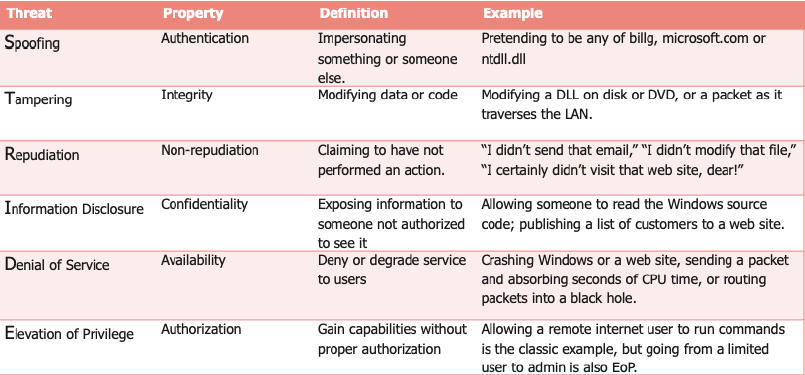
\includegraphics[width=1\linewidth]{../img/stride.png}
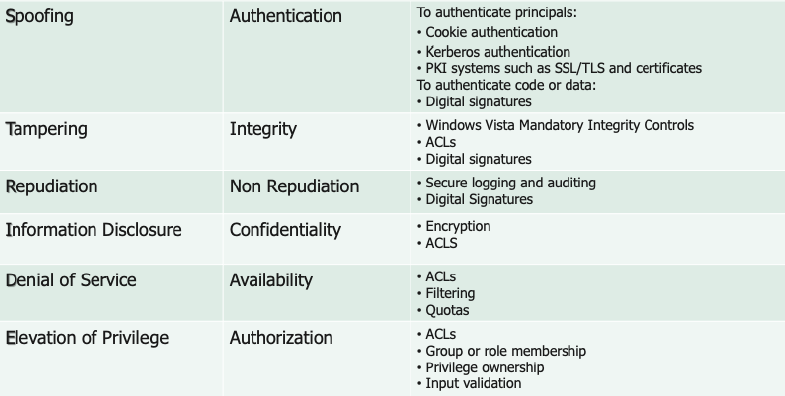
\includegraphics[width=1\linewidth]{../img/stride_mitigation.png}
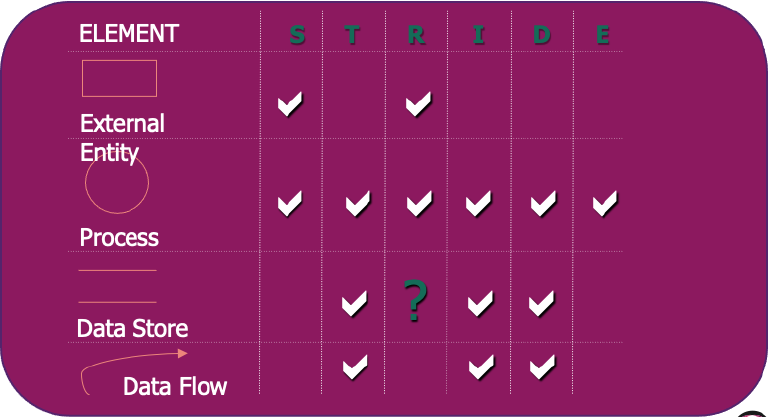
\includegraphics[width=1\linewidth]{../img/stride_mapping.png}\\
\columnbreak

\subsection{Attack Trees in context}
\begin{itemize}
    \item Very useful for developing one threat where mitigation is not obvious
    \item Complement a threat model
    \item Can start a threat modeling
    \item Can be used in teams
    \item Often generate good discussions
\end{itemize}

